\documentclass[10pt]{seminar} 

\renewcommand{\baselinestretch}{1}

\usepackage{amsmath}

\renewcommand{\printlandscape}{\special{landscape}}

\usepackage{ulem}



\input{seminar.bug}

%\usepackage{fancybox}

\usepackage{epsfig}

%\usepackage{times}


\usepackage{amssymb}

\usepackage{amscd}

\usepackage{graphics}

\usepackage{pstricks}

%\usepackage{chicago}

%\usepackage{fullpage}

\slideframe{none}

\begin{document}

\newtheorem{proposition}{Proposition}

\newtheorem{definition}{Definition}

\newtheorem{corollary}{Corollary}

\newtheorem{theorem}{Theorem}

\newtheorem{lemma}{Lemma}

\def\argmax{\mathop{\rm argmax}\limits}  


%\slideframe{Oval}

\sffamily 

\begin{slide}

 
 Let's show $f(x)$ is discontinuous at $x_o=3$
\begin{equation*}
 f(x)=\left\{ 
 \begin{array}{cc}
-1&\text{ if }x\geq 3\\
1 &\text{ if }x<3
 \end{array}
\right.
\end{equation*}
 
To show this using $(\delta, \epsilon)$ we show $\exists$ an $\epsilon>0$ such that for all $\delta>0$, we can find an $x$ such that $|x-x_o|<\delta$ such that $|f(x)-f(x_o)|\geq\epsilon$.  \textit{In other words, we can't find a $\delta>0$ such that $x$ within $\delta$ of $x_o$ implies that $f(x)$ is within $\epsilon $ of $f(x_o)$.}

\ \\ $|x-x_o|<\delta$ implies $|x-3|<\delta$, or $x\in (3-\delta, 3+\delta)$. Let's choose $\epsilon=2$, and consider \textit{any} $\delta>0$. Let $x^\prime=3-{\delta\over 2}\in (3-\delta, 3+\delta)$.  Then  $|f(x^\prime)-f(x_o)|=|1-(-1)|=2\geq \epsilon$. $\Box$




\newslide

\begin{center}

The derivative
 \end{center}
 
 \newslide
 
Lines and slopes

\ \\A line can be represented by the equation $y=a*x+b$, with $a$ being the slope and $b$ the $y-$intercept

\ \\For any points on the line, $(x_o, y_o)$ and $(x_1, y_1)$, we have $a={{y_1-y_o}\over{x_1-x_o}}$

\begin{center}
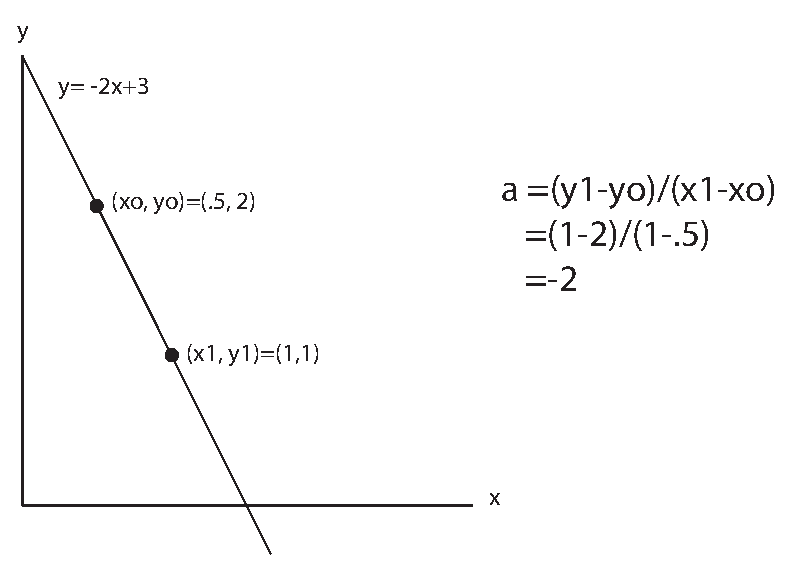
\epsfig{file=slope.eps, scale=.5}
\end{center}

\newslide

The \textit{slope of the curve} $f(x)$ at point $P$ is the limit of the slope of the line between $Q$ and $P$ as $Q\rightarrow P$

\begin{center}
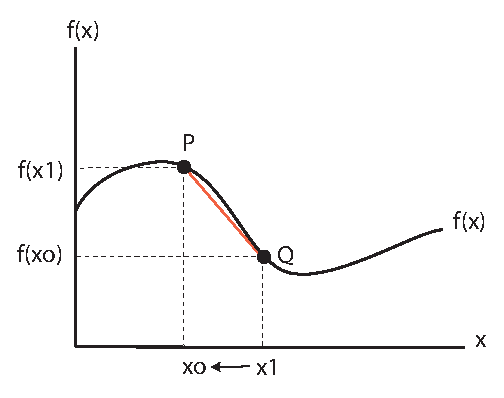
\epsfig{file=slopeCurve.eps, scale=.75}
\end{center}

\newslide

The \textit{slope of the curve} $f(x)$ at point $P$ is the limit of the slope of the line between $Q$ and $P$ as $Q\rightarrow P$

\ \\$P=(x_o, f(x_o))$ and $Q=(x_1, f(x_1))$; we'll write $x_1=x_o+h$ so that we have $x_1\rightarrow x_o$ as $h\rightarrow 0$

\ \\We now have $$P=(x_o, f(x_o)) \hbox{ and }Q=(x_o+h, f(x_o+h))$$ To find the slope of $f(x) $ at point $P$ we want to find the slope of the line between $P$ and $Q$ as $h\rightarrow 0$

\newslide
\ \\We now have $$P=(x_o, f(x_o)) \hbox{ and }Q=(x_o+h, f(x_o+h))$$ To find the slope of $f(x) $ at point $P$ we want to find the slope of the line between $P$ and $Q$ as $h\rightarrow 0$. This slope is:


$${{y_1-y_o}\over{x_1-x_o}}= {{f(x_o+h)-f(x_o)}\over{x_o+h-x_o}}$$

\ \\The slope of the curve $f(x)$ at the point $(x_o, f(x_o))$ is the \textit{derivative of $f$ at $x_o$}, or $f^\prime(x_o)$:

$$f^\prime(x_o)=\lim_{h\rightarrow 0}{{f(x_o+h)-f(x_o)}\over{h}}$$

\newslide

Alternative notation

\ \\The derivative $f^\prime(x)$ is the \textit{rate of change} of $f$ at $x$; as $x$ moves a little it tells us how much $f(x)$ moves in response

\ \\ \begin{center}
derivative $\Leftrightarrow$ slope $\Leftrightarrow$ rate of change $\Leftrightarrow$ gradient

\ \\$f^\prime(x)$ $\Leftrightarrow$ ${{dy}\over {dx}}$ $\Leftrightarrow$ $\lim\limits_{\Delta x\rightarrow 0}{{\Delta y}\over{\Delta x}}$ $\Leftrightarrow$ ${{d}\over{dx}} f(x)$
\end{center}

\newslide

Example: We'll use the formula $f^\prime(x_o)=\lim_{h\rightarrow o}{{f(x_o+h)-f(x_o)}\over{h}}$ to find the derivative of $f(x)=x^2-5x$

$$\lim_{h\rightarrow 0} {{(x+h)^2-5(x+h)-x^2-5x}\over{h}}$$

$$\lim_{h\rightarrow 0} {{x^2+2xh+h^2-5x-5h-x^2+5x}\over{h}}$$

$$\lim_{h\rightarrow 0} {{2xh+h^2-5h}\over{h}}$$

$$\lim_{h\rightarrow 0} {{2x+h-5}}$$

$$\mathbf{2x-5}$$

\newslide

A derivative of a function at $x$ is an approximation of the function by a straight line at $x$; sometimes such an approximation doesn't exist

\ \\For a function to be differentiable at a point, it must be continuous at that point
\ \\A differentiable function is differentiable at every point; it must be continuous, though continuous functions may not be differentiable

Example: $y=|x|$ at $x=0$

$$\lim_{h\rightarrow 0}{{|0+h|-|0|}\over{h}}$$

$$\lim_{h\rightarrow 0}{{|h|}\over{h}}$$

When $h\uparrow 0$ this equals $-1$.  When $h\downarrow 0$ this equals 1. The limit doesn't exist.

\newslide Useful rules

\begin{itemize}
\item Straight line rule: If $f(x)=ax+b  $ then $f^\prime(x)=a$

\item Power rule: if $f(x)=x^n$ then $f^\prime(x)=n x ^{n-1}$

\item Combination rule:  If $f(x)=a f_1(x)+b f_2(x)$ for $a, b\in \mathbb{R}$ then $f^\prime(x)=a f_1^\prime(x) +b f_2^\prime(x)$

 \end{itemize}

\newslide

Derivatives in politics and political economy

\ \\The 1-dimensional spatial model

\begin{itemize}
\item The policy space is $\mathbb{R}$
\item A person (voter?)  has an ``ideal point" $p\in \mathbb{R}$
\item Person prefers policies that are closer to his/her ideal point: receives utility  from policy $x$ that is $u(x)=-|x-p|$
\item Since this isn't differentiable (and for other reasons), we may assume that 
\end{itemize}
$$u(x)=-(x-p)^2$$

\newslide
$$u(x)=-(x-p)^2$$

$$u^\prime(x)=2p-2x$$

\vspace{.5in}
\begin{center}
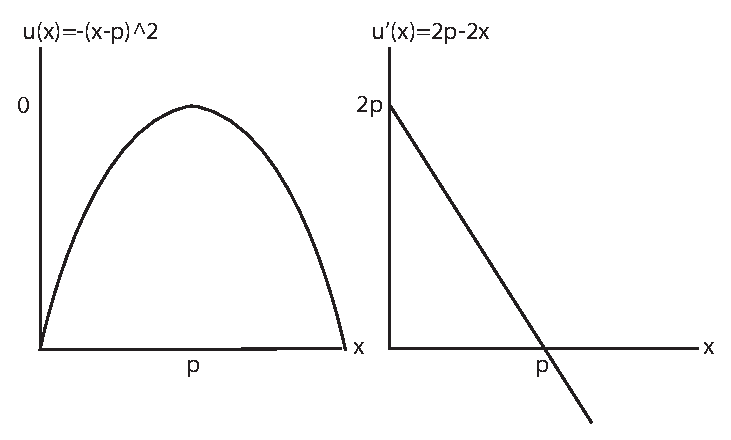
\epsfig{file=quad.eps, scale=.65}
\end{center}

\newslide

Tax rates

\ \\Suppose consumption of a good is given by $c=1-2t$, so that if $t=0$, 1 unit will be consumed; if $t\geq {1\over 2}$ then 0 units will be consumed.

\ \\The government receives revenues equal to (consumption * tax rate), $R=c*t=t(1-2t)$, or $$R=t-2t^2$$

\ \\If we want to see how revenues change as a function of the tax rate we take $$R^\prime=1-4t$$

\newslide

Revenues $$R=t-2t^2$$ $$R^\prime=1-4t$$

\vspace{.5in}
\begin{center}
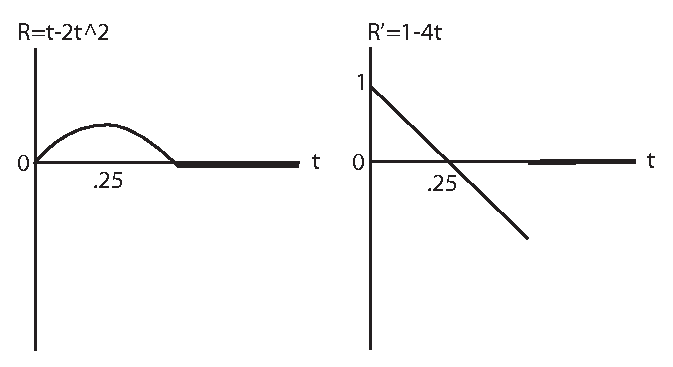
\epsfig{file=rev.eps, scale=.65}
\end{center}

\newslide
\begin{center}

Methods of differentiation, critical points, and optimization
 \end{center}
 
 \newslide
The product rule:  Let $u$ and $v$ be functions of $x$.  Then $${d\over{dx}}uv=v{{du}\over{dx}}+u{{dv}\over{dx}}$$

\ \\Example: Let $$f(x)= (1-20x^2)({1\over x}+2)$$ Find $f^\prime(x)$

\newslide
The quotient rule:  Let $u$ and $v$ be functions of $x$.  Then $${d\over{dx}}\left({u\over v}\right)={\left({v{{du}\over{dx}}-u{{dv}\over{dx}}}\right) / {v^2}}$$

\ \\Or: ``Low D high minus high D low, square the bottom and away we go!"

\ \\Example: Let $$f(x)= {{3x+a}\over{x^2+b}}$$ Find $f^\prime(x)$


\newslide
The composite function rule (aka the chain rule): Let $f(x)=g(h(x))$. Then $$f^\prime(x)=g^\prime(h(x))\cdot h^\prime(x)$$


\ \\Example 1: Find $f^\prime(x)$ for $$f(x)=({5\over x}+2x^2)^2$$ 

\ \\Example 2: Find $f^\prime(x)$ for   $$f(x)={1\over{g(x)}}$$ Does this look familiar?

\newslide

An example with voter preferences

\ \\Suppose that a voter has ideal point $v\in \mathbb{R}$, and receives utility from a policy $x$ equal to $$u(x)=-(v-x)^2$$

\ \\Now suppose that there is a politician with ideal point $p$, and that the politician chooses a policy that is the average of his own ideal point and his party's platform, $P$, so that policy $x={{p+P}\over 2}$.  How does the voter's utility change as a function of the candidate's ideal point, $p$? \\(In other words, find ${du}\over {dp}$)

\newslide

Monotonic functions: functions that are either \textit{strictly increasing} or \textit{strictly decreasing}

\ \\Strictly increasing: If $x_2>x_1$ then $f(x_2)>f(x_1)$
\ \\Strictly increasing: If $x_2>x_1$ then $f(x_2)<f(x_1)$


\ \\If $f^\prime(x)>0$ for all $x$, then $f$ is strictly increasing; \\however this is stronger than we need for a function to be strictly increasing (e.g. $f(x)=x^3$)

\ \\If $f^\prime(x)\geq 0$ for all $x$ and $f^\prime(x)=0$ for only a finite number of $x$, then $f$ is strictly increasing (with strictly decreasing proved similarly)

\newslide
Inverse functions

\ \\Let $f(x)$ be monotonic.  Then for any $y$, $f(x)=y$ has at most one solution. If the solution is written $x=g(y)$, then $g$ is the \textit{inverse function} of $f$, or $$f(g(y))=y \hbox{ and }g(f(x))=x$$


\ \\Example 1:  Let $f(x)=1-x^2$; what is the inverse function of $f$? 
$$y=1-x^2$$
$$x^2=1-y$$
$$x=(1-y)^{1\over 2} = g(y)$$

\ \\The inverse function always reflects the function about the $45^\circ$ line!

\newslide

\ \\Example 1:  Let $f(x)=x^3$; what is the inverse function of $f$?

\begin{center}
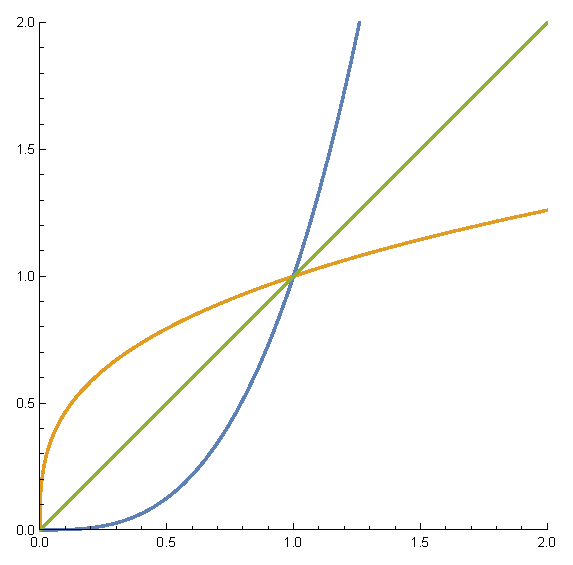
\epsfig{file=inv1.eps, scale=.6}

\end{center}
\newslide
\ \\Example 2: Let $f(x)=x^{-1}+5$; what is the inverse function of $f$?
\begin{center}
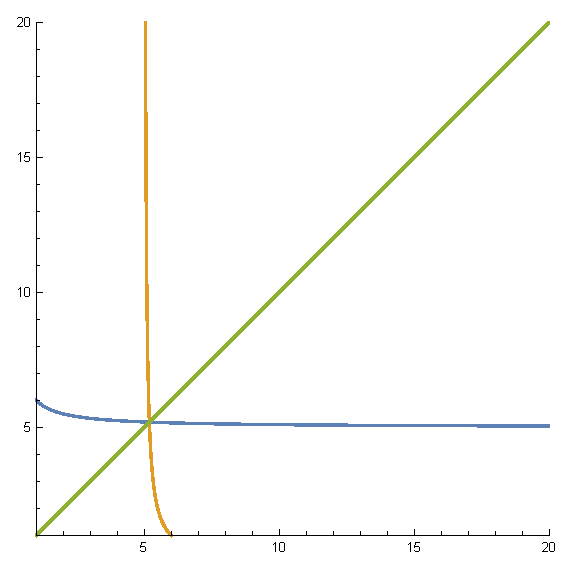
\epsfig{file=inv2.eps, scale=.6}

\end{center}


\newslide 
The inverse function rule

\ \\If $f$ is monotonic with inverse function $g$, and for a given $x$, $f$ is differentiable and $f^\prime(x)\not=0$, then $$g^\prime(y)={1\over {f^\prime(x)}}$$


\ \\This gives us another technique for differentiating things; we could calculate $f^\prime$ directly, or we could calculate $1\over{g^\prime}$

\newslide
Critical points

\ \\If $f^\prime(x)=0$ then $x$ is called a \textit{critical point}

\begin{itemize}
\item Maximum
\item Minimum
\item Inflection point
\end{itemize}

\begin{center}
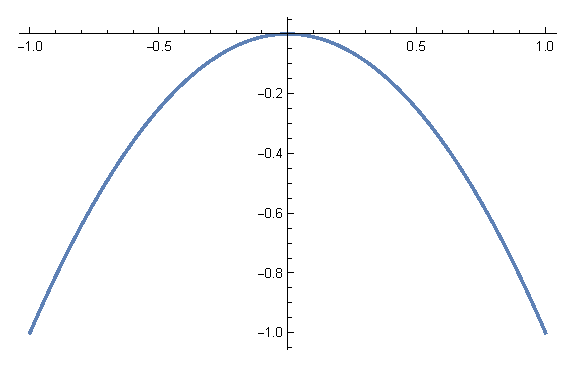
\epsfig{file=max.eps, scale=.32} 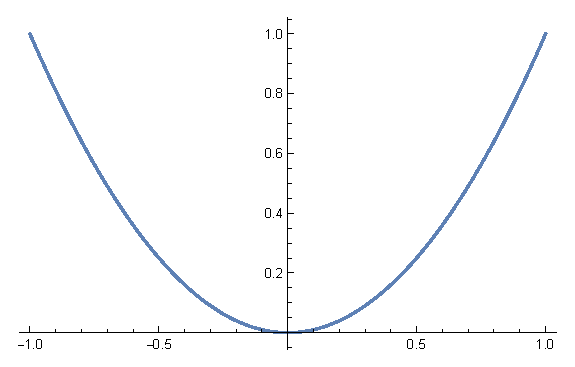
\epsfig{file=min.eps, scale=.32} 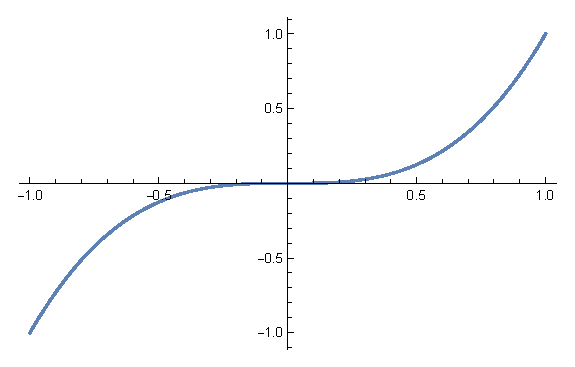
\epsfig{file=inflect.eps, scale=.32}
\end{center}

\newslide

One of the main things we use calculus for is to identify and classify critical points

\begin{enumerate}
\item Find $f^\prime(x)$
\item Find the set of $x$ such that $f^\prime(x)=0$
\item Intuitively, if $f^\prime(x)$ changes from negative to positive around $x$, then $x$ is a minimum; if it changes from positive to negative then $x$ is a maximum; if it does neither then it's a point of inflection
\item Always remember that without more knowledge of $f$, all we know is that $x$ is a \textit{local} maximum or minimum (or an inflection point); we can't assume that it maximizes or minimizes our function globally
\end{enumerate}

\newslide

The second derivative

If $f^\prime$ is itself differentiable, then $f$ is \textit{twice differentiable}, and $f^{\prime\prime} = {{d^2y}\over{dx^2}}$ is the \textit{second derivative}

\begin{itemize}
\item Suppose that $f^{\prime\prime}(x)$ is positive at some point $x$
\item This means that the \textit{slope of the slope} of $f$ is increasing at $x$
\item This means that either:

\begin{itemize}

\item If $f$ is increasing then it's increasing at an increasingly faster rate at $x$
\item If $f$ is decreasing then it's decreasing at an increasingly slower rate at $x$
\item If $f$ is flat then it's increasing as $x$ increases

\end{itemize}
\item In all of these cases, $f$ lies above its tangent
\end{itemize}

\newslide

\begin{itemize}

\item[A] If $f$ is increasing then it's increasing at an increasingly faster rate at $x$
\item[B] If $f$ is decreasing then it's decreasing at an increasingly slower rate at $x$
\item[C] If $f$ is flat then it's increasing as $x$ increases

\end{itemize}

\vspace{.2in}
\begin{center}
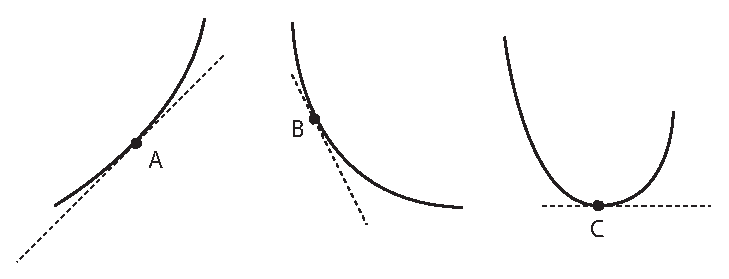
\epsfig{file=convex.eps, scale=.75}
\end{center}

\newslide

The second derivative test

\begin{itemize}
\item For any critical point, $x^*$, calculate $f^{\prime\prime}(x^*)$

\begin{itemize}
\item If $f^{\prime\prime}(x^*)>0$ then $x^*$ is a local minimum
\item If $f^{\prime\prime}(x^*)<0$ then $x^*$ is a local maximum

\item If $f^{\prime\prime}(x^*)=0$ then we don't know what $x^*$ is; we have to examine our function around $x^*$

\end{itemize}

\item $f^\prime(x)=0$ is our first-order condition; conditions on $f^{\prime\prime}$ are our second-order conditions

\end{itemize}


\ \\Find and classify the critical points of $x^3-3x$, and then use this information to plot out the function

\newslide

Global maxima (minima work the same way)

\ \\If a local maximum $x^*$ has the additional property that $f(x^*)\geq f(x)$ for all $x\in \mathbb{R}$ then $x^*$ is a global maximum %was the local maximum we just found a global maximum?

\ \\Important points about global maxima that we will use shortly

\begin{itemize}
\item Suppose that $g(x)=H(f(x))$ where $H$ is a \textit{strictly increasing function}.  Then if $f$ has a global maximum at $x^*$, $g(x)$ also has a global maximum at $x^*$
\begin{itemize}
\item If $f(x^*)\geq f(x)$ for all $x$, then $H(f(x^*))\geq H(f(x))$ for all $x$, since $H$ is a strictly increasing function
\item It can be useful to take a log; if $x^*$ globally maximizes log$(f(x))$ then $x^*$ also maximizes $f(x)$
\end{itemize}

\item If $x^*$ is the global max of $f(x)$ then $x^*$ is the global minimum of $-f(x)$
\end{itemize}

\newslide
Boundary conditions \& asymptotes

\ \\ If the domain of a function is bounded, it may be the case that a global maximum is attained at one of the boundaries, even when the first-order condition at that point is not satisfied; use common sense and try to have a sense of what your function looks like -- some problems are best solved without calculus.

\ \\The extreme value theorem:  any continuous function on a closed and bounded interval attains a global maximum \& minimum

\ \\Some functions tend to a straight line for all very large values of $|x|$ and / or  $|y|$; it can be useful to know this

\begin{itemize}
\item $y={1\over x}$ ($x>0$) has a $x-$ and $y-$ asymptotes equal to the axes
\item What are the asymptotes for $y=x-{1\over x}$? %has asymptotes equal to the y axis and the line y=x
\end{itemize}

\newslide Convexity and concavity

\begin{itemize}
\item Convex and concave functions guarantee that local optima are global optima, and are commonly encountered
\item A set is \textit{convex} if the line segment connecting any two points in the set is entirely contained within the set
\item A function is convex if the set of all points on or above the graph is a convex set

\end{itemize}
\begin{center}
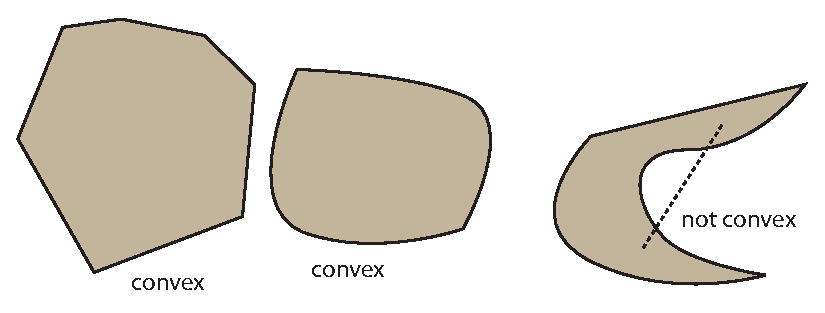
\epsfig{file=convexSet.eps, scale=.65}
\end{center}

\newslide

$f$ is a convex function if and only if for all real numbers $A, B$ and all $0\leq \alpha \leq 1$, 
$$\alpha f(A)+(1-\alpha)f(B)\geq f(\alpha A+(1-\alpha)B)$$

\begin{center}
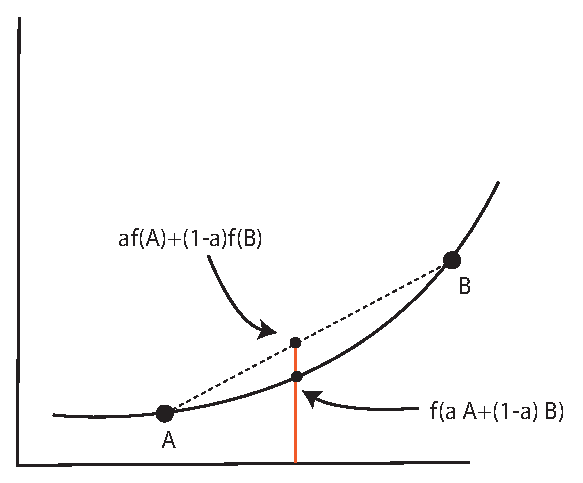
\epsfig{file=convexFunction.eps, scale=.65}
\end{center}

\newslide

Convex functions need not be differentiable (e.g. $y=|x|$); the ones we generally encounter are


\begin{itemize}
\item If $f$ is twice differentiable, then $f$ is convex if and only if $f^{\prime\prime}\geq 0$ for all $x$

\item If $f$ is convex \& differentiable then
\begin{itemize}
\item There is either no global minimum, one global minimum, or an interval of global minima
\item There are no local minima that are not global minima
\item Important: if $f^\prime(x^*)=0$ then $x^*$ is a global minimum
\end{itemize}
\item $f$ is \textit{strictly convex} if $\alpha f(A)+(1-\alpha)f(B)> f(\alpha A+(1-\alpha)B)$ when $\alpha\in(0, 1)$
\end{itemize}

\newslide

$f$ is \textit{concave} if and only if $-f$ is convex: the set of all points on or below $f$ is convex

\begin{itemize}
\item If $f$ is twice differentiable then $f$ is concave if and only if $f^{\prime\prime}\leq 0$ for all $x$

\item Important: if $f$ is concave and $f^\prime(x^*)=0$ then $x^*$ is a global maximum

\end{itemize}

\newslide

A simple model of effort; I can exert effort $e$ and receive some benefit $B*e$, but I must pay cost $c*e^2$, with $B, c>0$

$$U(e)=Be-ce^2$$

\begin{itemize}
\item This function is concave: $U^\prime=B-2ce$ and $U^{\prime\prime}=-2c<0$

\item It has a global maximum at $e^*={{B}\over {2c}}$

\item \textit{Comparative statics}: given an optimizing point such as this, how does this optimum vary as other parameters of the problem vary?

\end{itemize}
 $${\partial e^* \over {\partial B}}={{1}\over{2c}}>0$$

 $${\partial e^* \over {\partial C}}=-{{B}\over{2c^2}}<0$$

\newslide

The exponential function

\begin{itemize}
\item The number $e$ is defined by $$e=\lim_{n\rightarrow\infty}(1+{1\over n})^n \approx 2.7183$$
\item $y=e^x$ is the \textit{exponential function}
\item ${d\over{dx}}e^x=e^x$
\end{itemize}

\newslide
Natural logarithms

\begin{itemize}
\item The natural logarithm of $x$ is the log to base $e$ of $x$ 
\item (If $\ln(x)=y$ then $e^y=x$)
\item ${d\over{dx}}\ln(x)={1\over x}$
\end{itemize}
\vspace{.2in}
Recall your log facts:


\begin{itemize}
\item $\ln (x^c)=c\ln x$
\item $\ln (xw)=\ln x+\ln w$
\item $\ln ({x\over w})=\ln x-\ln w$
\end{itemize}

\newslide

Application: Optimizing work versus play

\ \\Suppose that I have 10 hours in which to either work or play $w+p=10$

\ \\I receive a payoff from any given mixture of these activities that looks like the following:

$$U(w, p)=w^\alpha p^{1-\alpha},$$ for some $\alpha\in (0, 1)$.  Notice that if either $w=0$ or $p=0$ my utility is zero; some work is required to survive, but without some play \textit{what is the point of living}?

\ \\$\alpha$ captures the responsiveness of my well-being to a change in work (holding play constant)

\newslide

While this looks like a choice over 2 things, it's really a choice over 1: Letting $p=10-w$ we get


$$U(w)=w^\alpha (10-w)^{1-\alpha},$$ for some $\alpha\in (0, 1)$. What is the $w$ (and consequently, the $p$ that maximizes this?

\ \\This is hard to solve explicitly, but we can take a log of this function:

$$U(w)=\alpha \ln(w)+(1-\alpha)\ln(10-w)$$

\ \\What's the solution? How does it vary as a function of $\alpha$? Is utility concave?



\end{slide}



\end{document}








